\RequirePackage{plautopatch}  % pLaTeX または upLaTeX のとき
%\documentclass[uplatex,dvipdfmx,titlepage,a4j]{jsarticle}% upLaTeX のとき
\documentclass[dvipdfmx,titlepage,a4j]{jsarticle}  % pLaTeX のとき
\usepackage{listings,jvlisting}
\usepackage{amsmath,amssymb}
\usepackage{graphicx}
\usepackage[yen]{okuverb}
\usepackage{r04ec-exp}
\usepackage{here}
\usepackage{ascmac}
\usepackage{fancybox}
\usepackage{fancyvrb}
\usepackage{fancyhdr}
\usepackage{lastpage}
\usepackage{cases}

\fancypagestyle{foot}
{
\fancyhead[C]{電子回路設計・製作}
\fancyfoot[C]{\thepage / \pageref{LastPage}}
\renewcommand\headrulewidth{0.4pt}
}

%ここからソースコードの表示に関する設定
\lstset{
  language={C++},
  basicstyle={\ttfamily},
  identifierstyle={\small},
  commentstyle={\smallitshape},
  keywordstyle={\small\bfseries},
  ndkeywordstyle={\small},
  stringstyle={\small\ttfamily},
  frame={tb},
  tabsize={2},
  breaklines=true,
  columns=[l]{fullflexible},
  numbers=left,
  xrightmargin=0zw,
  xleftmargin=3zw,
  numberstyle={\scriptsize},
  stepnumber=1,
  numbersep=1zw,
  lineskip=-0.5ex
}

\renewcommand{\lstlistingname}{リスト}
%ここまでソースコードの表示に関する設定

\title{電子回路設計・製作 DTMF信号音エミュレータ}
% 学年・番号
\grade{4年42番}%
% 氏名
\author{鷲尾 優作}
% 班(後期は班に分かれて実験をする.そのときは,ここに班番号を記入する.)
\team{}
% 提出日
\date{2022年10月6日}
% 実験日
\expdate{2022年6月16日,23日,30日,7月7日,14日,21日,8月4日}
% 共同実験者
% グループに分かれて実験をするテーマでは,グループメンバーの番号名前を書く.
\coauthor{}
%
%記載例:
%\coauthor{%
%  2番 & 新潟 花子\\
%  11番 & 三条 次郎}
%%

\begin{document}
\pagestyle{foot}

\maketitle

\section{作品タイトル}
DTMF信号音エミュレータ
\section{構造}
図\ref{fig:dia.png}に作成した回路の構造を示す.
回路は,Arduino Uno R3をベースに作成した.表示器として,液晶ディスプレイとLEDを備え,信号音を出力するスピーカー,その増幅回路を搭載している.
携帯電話と同一な,4×4キーパッドを搭載しており,この入力に応じて出力音を選択することができる.

\begin{figure}[H]
  \centering
  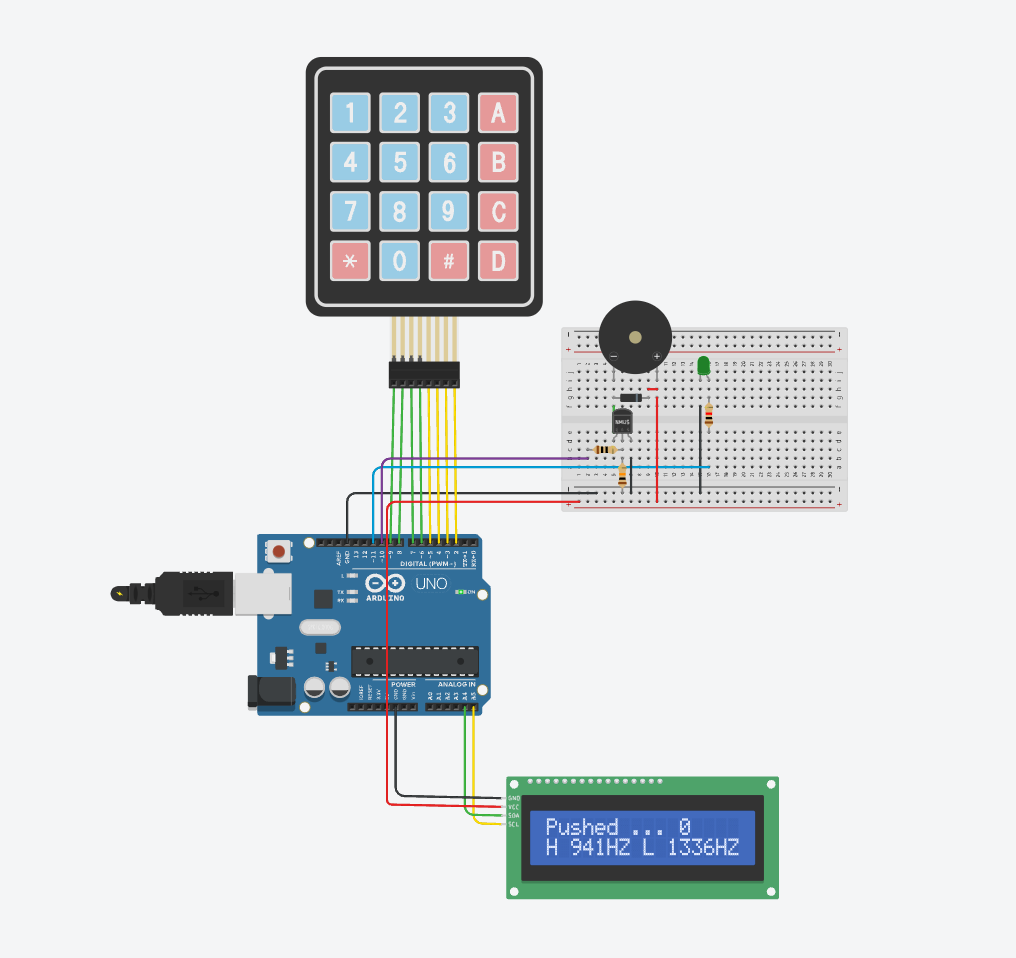
\includegraphics[width=6cm]{../fig/dia.png}
  \caption{DTMF信号音エミュレータ作品図}
  \label{fig:dia.png}
\end{figure}

\section{動作原理}
DTMF信号は,0から9までの数字,*,\#,A,B,C,Dの記号の計16種類を,
低群・高群の周波数の信号音で表現するものである.電話機による電話番号の送出などに用いられた技術であり,
人間の可聴音であるためピポパという音として認識することが可能である.

今回の実験では,TinkerCADにキーパッドのモデルが用意されていたことから着想し,この送信音を再現することを目的とした回路設計を行なった.

信号音を発生させるのは,Arduino Uno R3のに接続した圧電スピーカである.
このスピーカは,Arduinoのピン10に出力されるPWM信号を入力として,音を発生させる.
PWM信号は,キーパッドの入力に応じて,Arduinoのプログラムによって周波数が決定され,出力される.
NchFETを使った簡易な増幅回路を備えており,ピンそのものへの負荷を軽減している.
また,動作を確認するためI2C接続の液晶ディスプレイと単色の砲弾型LEDを搭載している.
液晶ディスプレイにはキーパッドの入力番号及び出力中の周波数が表示される.

\section{ハードウェア}
図\ref{fig:cir.png}に作成した回路の構造を示す.
\begin{figure}[H]
  \centering
  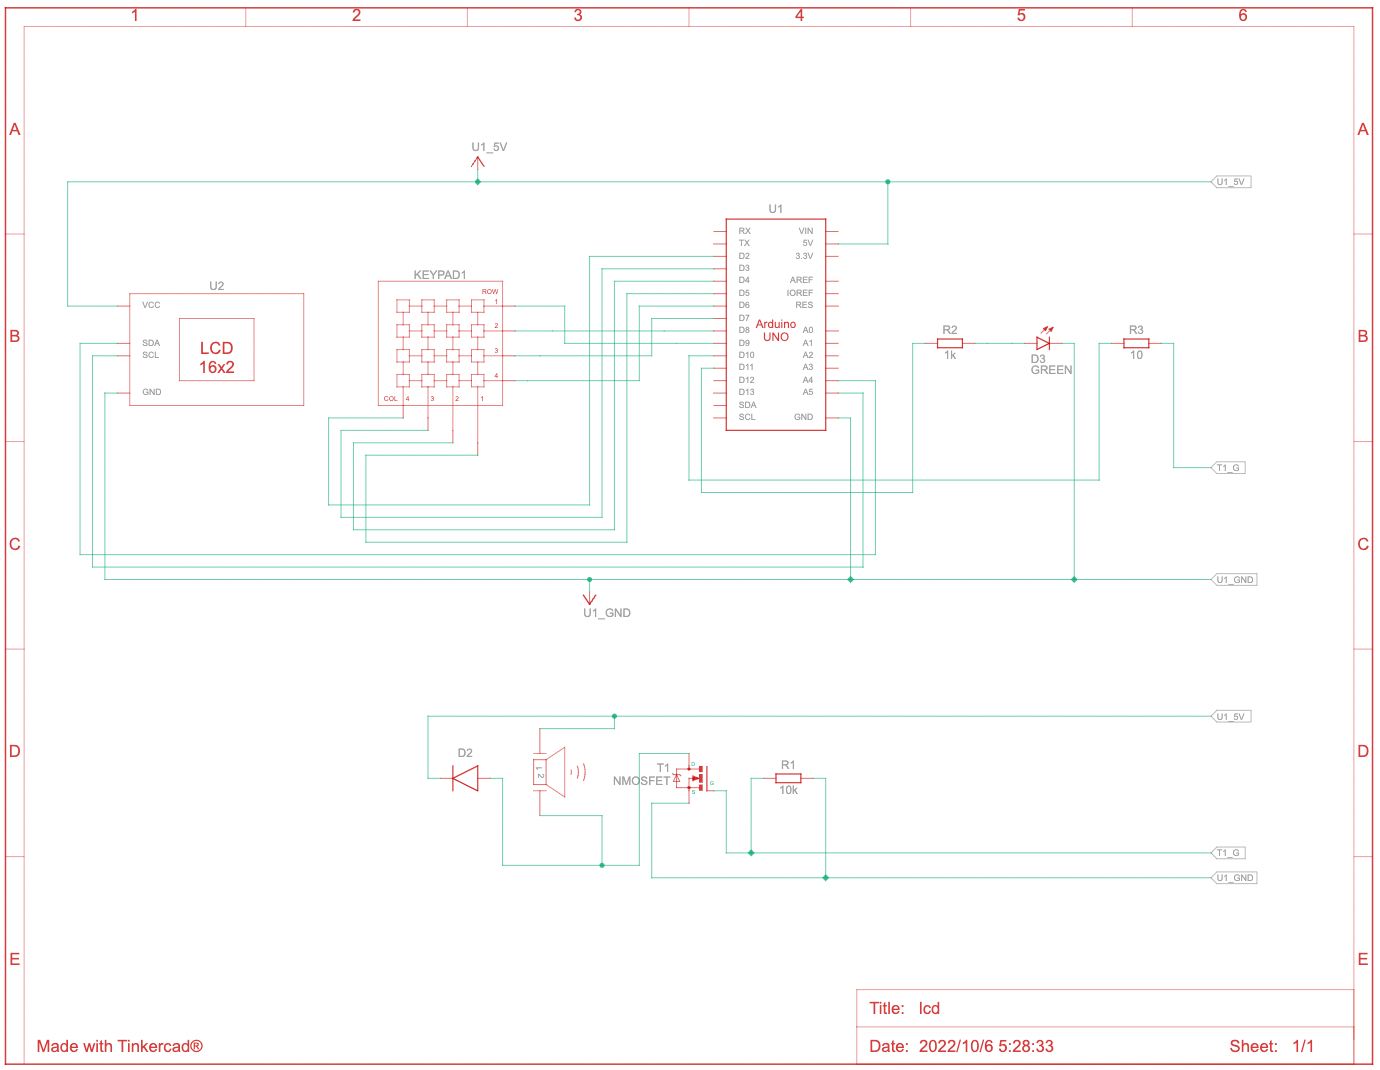
\includegraphics[width=10cm]{../fig/cir.png}
  \caption{DTMF信号音エミュレータ回路図}
  \label{fig:cir.png}
\end{figure}
表示器である液晶ディスプレイ,Arduino UNO とI2C接続により接続されている.
ArduinoのピンA4とA5に接続されており,信号通信を行うSDA,クロックであるSCL,及び電源線2本の計4本となる.

ピン10には,圧電スピーカが接続されている.
ピン10は,ArduinoのPWM出力に接続されており,このピンに出力されるPWM信号を入力として音を発生させる.
ArduinoUNOのチップであるATMega328PのGPIOの許容電流は20mAであり,
TinkerCADに用意されているスピーカーの詳しい仕様が不明であったため,
安全策としてピン10への負荷を軽減するためにNchFETを用いた増幅回路を搭載している.
また,同様にTinkerCADに用意されているNchFETの詳しい仕様や品番が不明であったため,
適当にゲート抵抗に10$\Omega$,ゲートソース間抵抗に10k$\Omega$を設定している.

キーパッドは,内部は縦横の4本ずつの接点を備えたスイッチである,
Arduinoのピン2から9に接続されており,特定のキースイッチが押されると,対応するピン間の電圧が0Vになる.

\section{ソフトウェア}
Arduino Uno R3のソフトウェアについて説明する.
図\ref{fig:flow.png}に作成した回路の構造を示す.
\begin{figure}[H]
  \centering
  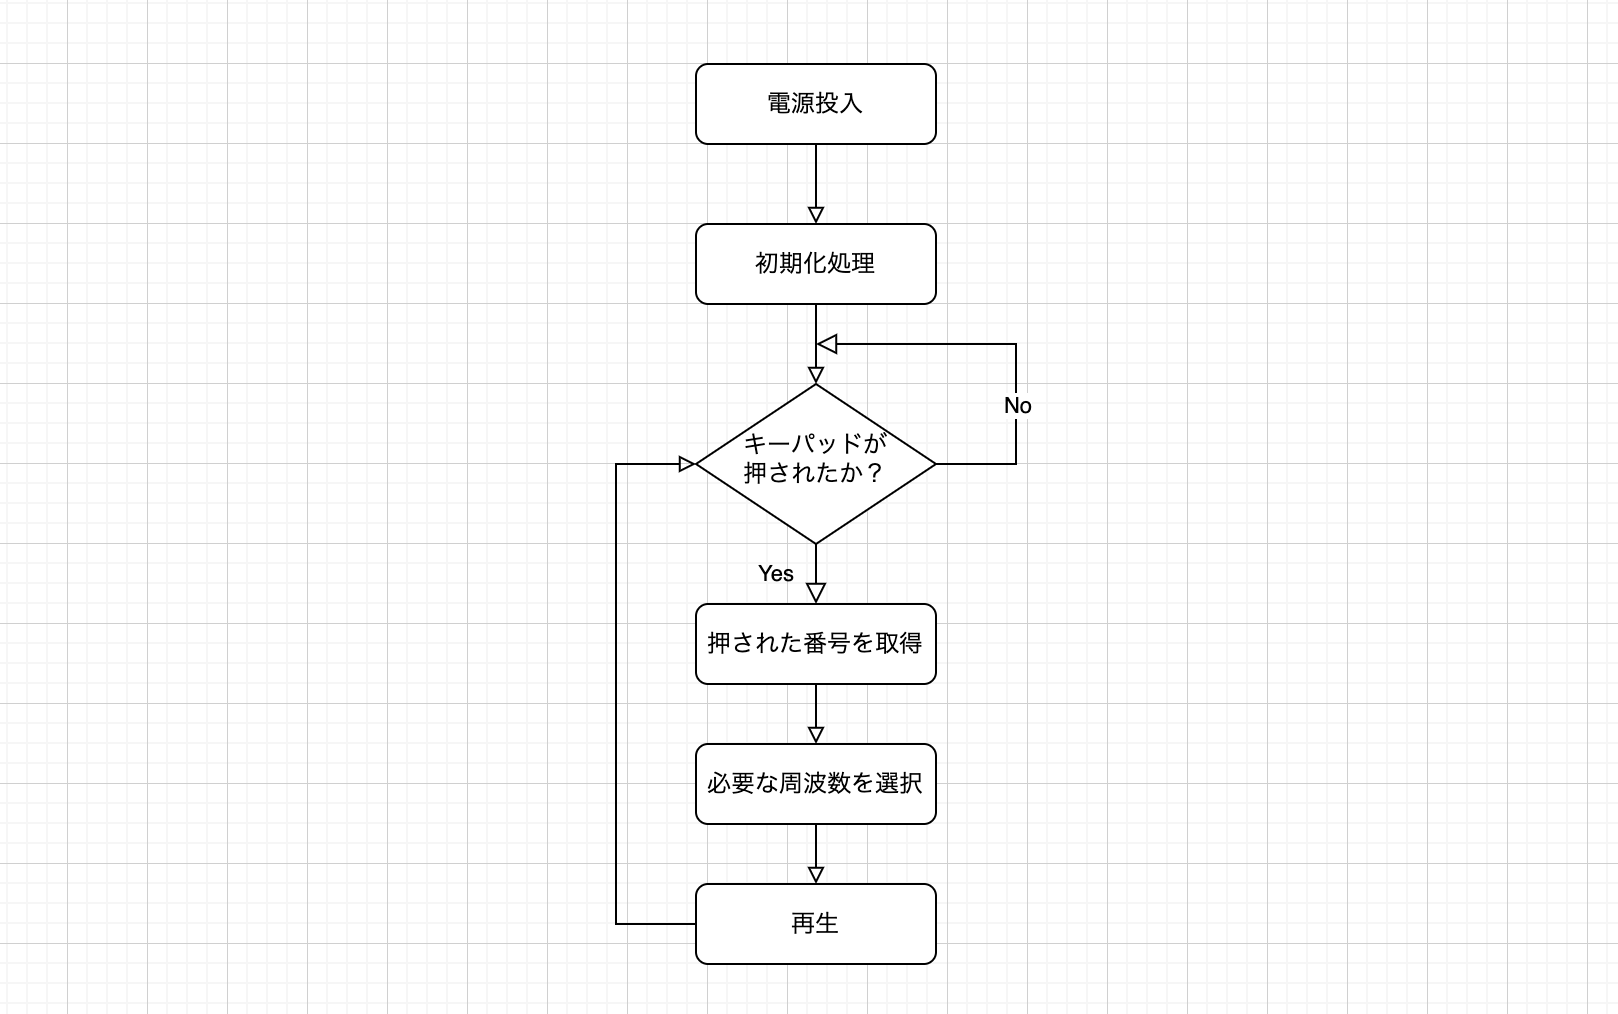
\includegraphics[width=10cm]{../fig/flow.png}
  \caption{DTMF信号音エミュレータフローチャート}
  \label{fig:flow.png}
\end{figure}
プログラム内ではKeypad.h,LiquidCrystal\_I2C.h,Wire.hを使用している.
キーパッドのピン設定については,KeyPad.hへの2次元配列の定義のみなので割愛する.

DTMF信号の各周波数はマクロ定義している.リスト\ref{code:macro}に示す.
\lstinputlisting[caption=dtmf.ino マクロ部,label=code:macro,firstline=5,lastline=13,firstnumber=5,]
{../dtmf.ino}

電源投入時の初期化処理を,リスト\ref{code:setup}に示す.
各ピンの出力設定,液晶ディスプレイの初期化を行なっている.
\lstinputlisting[caption=dtmf.ino 初期化部,label=code:setup,firstline=29,lastline=42,firstnumber=29,]
{../dtmf.ino}

LCDディスプレイの表示を担う関数をリスト\ref{code:lcd}に示す.
押されたキーの番号,及び出力中の周波数を引数として受け取り,それらを表示する.
\lstinputlisting[caption=dtmf.ino LCD関数部,label=code:lcd,firstline=44,lastline=55,firstnumber=44,]
{../dtmf.ino}

キー入力を受け付け再生するプログラムの一部をリスト\ref{code:key}に示す.
キー入力の文字列によってswitch文で分岐し,各キーに対応する周波数を出力する.
\lstinputlisting[caption=dtmf.ino 再生部,label=code:key,firstline=57,lastline=80,firstnumber=57,]
{../dtmf.ino}

最後に,main関数をリスト\ref{code:main}に示す.
main関数では,キー入力を受け付け,キー入力があれば,処理関数を呼び出す.
\lstinputlisting[caption=dtmf.ino メイン部,label=code:main,firstline=150,firstnumber=150,]
{../dtmf.ino}

\section{結果と今後の課題}
回路は想定通りの動作をし,キー入力に対応した周波数の音を出力することができた.
しかしながら,ArduinoUNOはシングルコアであるため,DTMF信号の出力周波数を決定する波形は同時に1つしか出力できない.
今回は信号音を聞くことに専念した設計とし,高速で交互に低音と高音を出力しているが,本来の伝送信号としては不適切である.
マルチスレッド処理が可能なICを用いるか,独立した2系統の回路的な処理系を設け,2スピーカーでそれぞれ音を出力する改良を加えたい.

\section{感想}
TinkerCADは設定されている素子の特性が明確になっていないため,回路の設計が難しかった.
DTMF信号というやや古いテーマ設定をしたが,わかりやすく,実装が容易であったので良い課題であったと思う.
Arduinoを2台同期することも考えたが,シュミレータの処理速度の問題があるため,今回は1台で完結させた.
KeyPad.hについては今回そのまま使用したが,あまり良いライブラリではない気がするので,今後は自作したい.

\begin{thebibliography}{99}
  \bibitem{ataka} 碓氷 小柳 梅田、実験テキスト「電子回路設計製作」、(2022年),
  \bibitem{wiki} Wikipedia、DTMF、https://ja.wikipedia.org/wiki/DTMF、(2022年),
\end{thebibliography}

\end{document}